% !TEX root = ../../main.tex

\section{Multicut}\label{sec:rw_multicut}

Segmentation is an important problem in computer vision as a first step
towards understanding an image. Many algorithms start with an over-segmentation
into superpixels, which are then clustered into ``perceptually meaningful''
regions.
Usually, the number of these regions is not known beforehand.

Recently, the multicut formulation~\cite{chopra_1993_mp}
(sometimes called \emph{correlation clustering}, \cite{bansal_2004_ml})
has become increasingly popular for unsupervised
image segmentation \cite{andres_2011_iccv,yarkony_2012_eccv,alush_2013_simbad}.

In this section we will give a brief overview of methods using multicut objectives
and will briefly introduce the multicut formulation.
The multicut and related work will be discussed extensively in \cref{ch:cgc} where
we propose a new solver for the such problems.

\paragraph{Problem Formulation:}
Given an edge-weighted region adjacency graph,
the problem is to find the segmentation which
minimizes the cost of the cut edges.
Therefore multicuts can be viewed as \emph{thresholding} w.r.t. close contours, while
naive thresholding will lead to inconsistencies 
(see \cref{fig:naive_thresholding} ).

Let $G=(V,E, \w)$ be a weighted region adjacency graph of
nodes $V$, representing superpixels,
and edges $E$.
%
The function $\w : E \rightarrow \mathbb{R}$ assigns a weight to each edge.
A positive weight expresses the desire that two adjacent nodes should
be merged, whereas a negative weight indicates
that these nodes should be separated into two different regions.
The \emph{multicut problem} can be written as a node labeling problem
\cite{bagon_2011_arxiv}:
%
\begin{align}
\argmin_{\Labels}
    \left\{
    \sum_{ e=(i,j) \in E}
        \w(e)
        \cdot \delta( \Labels_i \neq \Labels_j )
    \right\},
    \label{eq:multicut_primal_a}
\end{align}
%
where $\delta(a) = 1$ if $a$ is true and $0$ else.





\begin{figure}
\centering
\subfloat[Oversegmentation]{ \label{fig:naive_thresholding_a}
    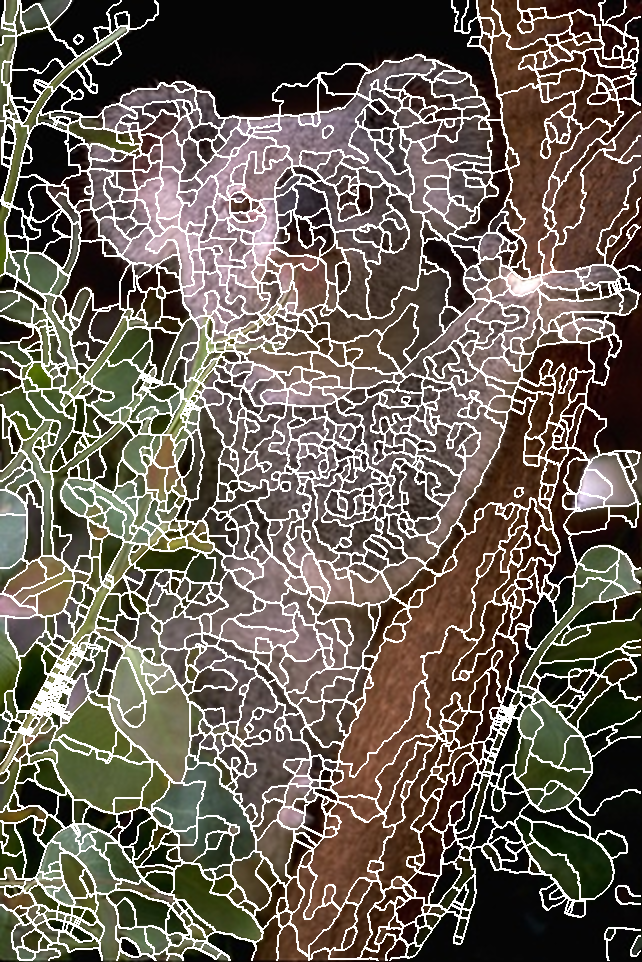
\includegraphics[width=0.25\textwidth]{fig/andres/0.png}
}
\subfloat[Oversegmentation]{  \label{fig:naive_thresholding_b}
    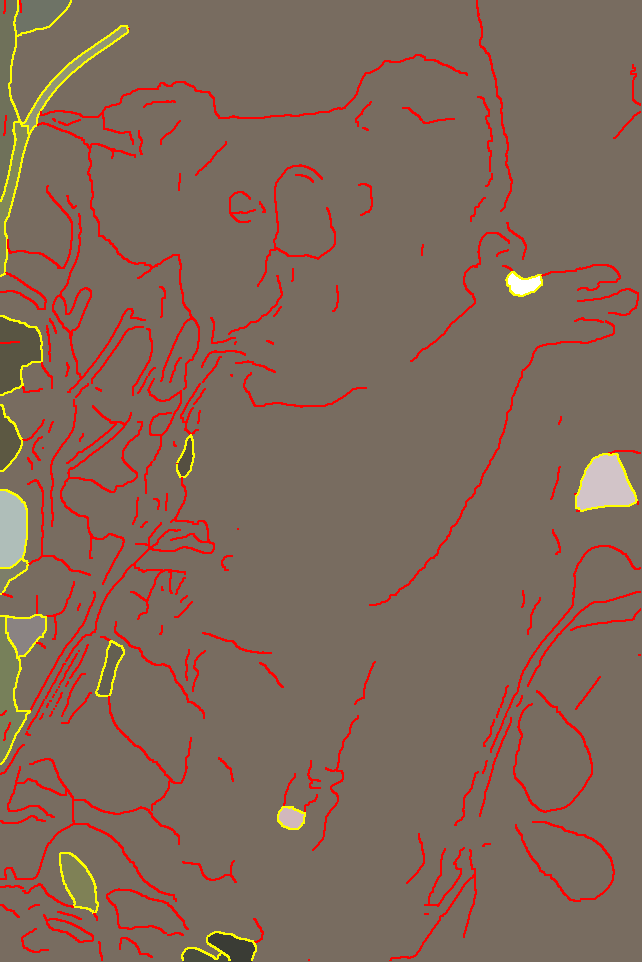
\includegraphics[width=0.25\textwidth]{fig/andres/1.png}
}
\subfloat[Oversegmentation]{  \label{fig:naive_thresholding_c}
    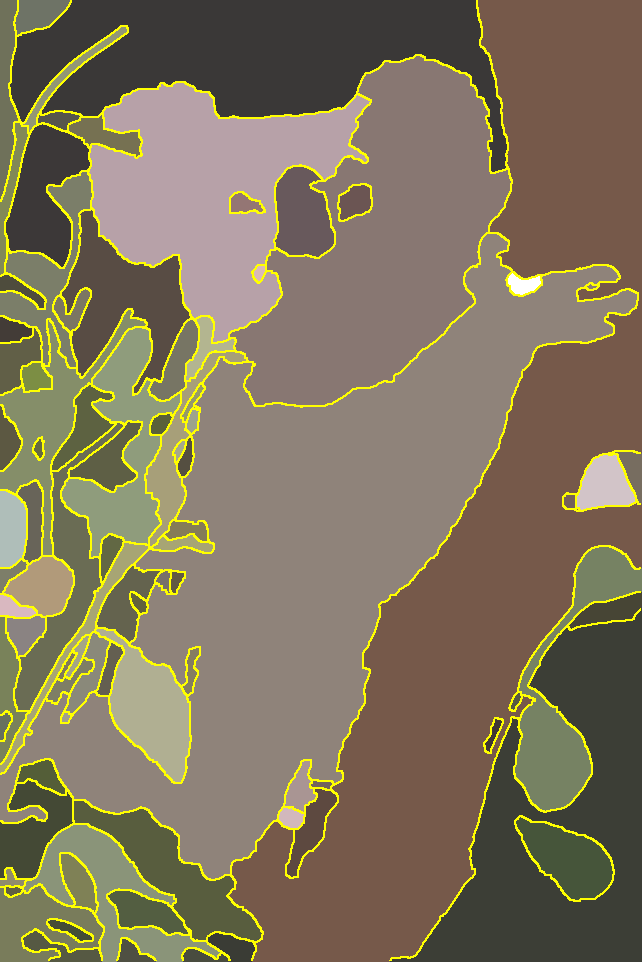
\includegraphics[width=0.25\textwidth]{fig/andres/2.png}
}
\addtocontents{lof}{%
    \vspace{1cm}
    \protect\centerline{%
        \protect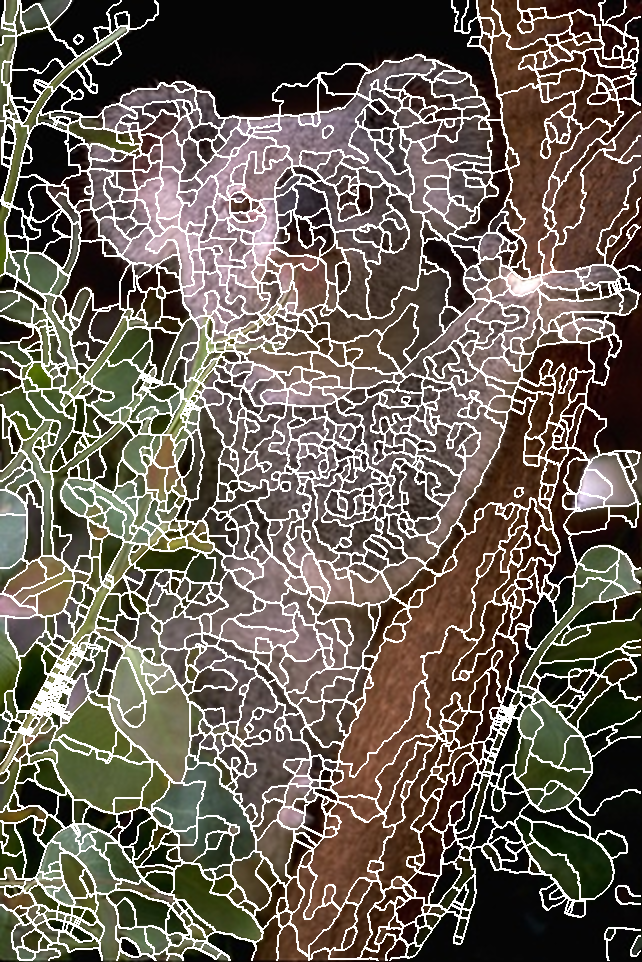
\includegraphics[width=.075\linewidth]{fig/andres/0.png}\hspace{0.2cm}
        \protect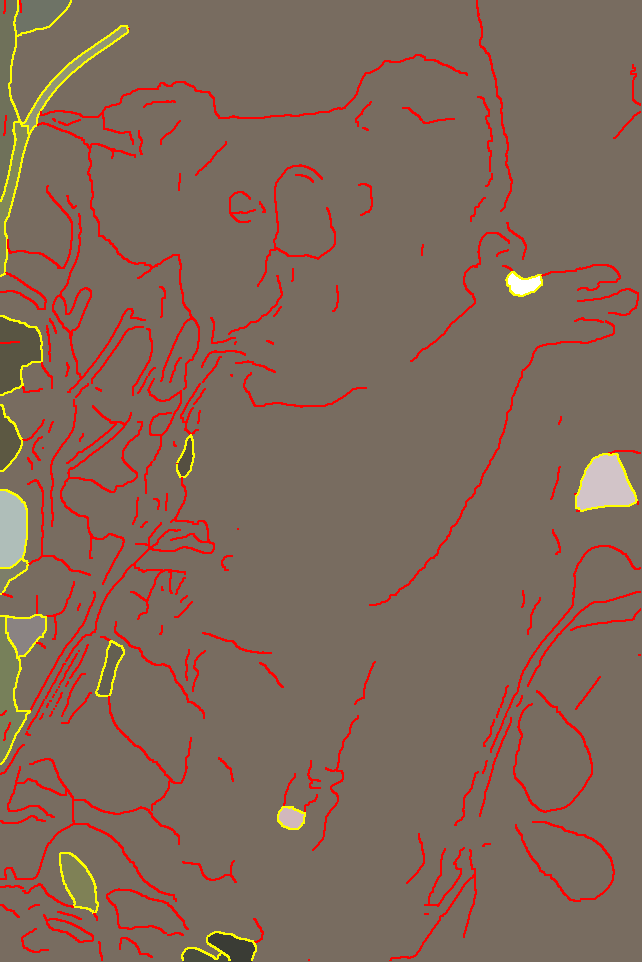
\includegraphics[width=.075\linewidth]{fig/andres/1.png}\hspace{0.2cm}
        \protect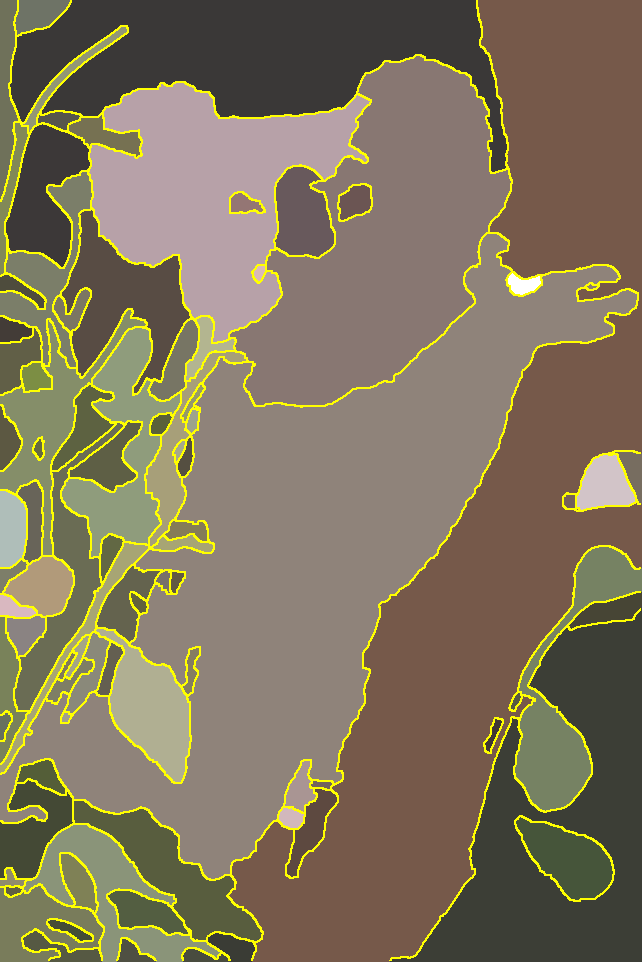
\includegraphics[width=.075\linewidth]{fig/andres/2.png} 
    }%
}%
\caption[Naive thresholding vs. multicuts]{
This figure has been taken from \cite{andres_2011_iccv} .
\Cref{fig:naive_thresholding_a} shows the oversegmentation of 
an image .
\Cref{fig:naive_thresholding_b} shows the result of naive thresholding..
Any inconsistent boundary is shown in red while consistent
boundaries are shown in yellow. 
\Cref{fig:naive_thresholding_c} shows the result with the multicut
constraints which lead to a meaningful segmentation.
} \label{fig:naive_thresholding}
\end{figure}


\citet{andres_2011_iccv} and \citet{kappes_2011_emmcvpr} use a
cutting plane approach where violated constraints are added
iteratively until no more violated constraints are found.


\begin{figure}
\centering
\subfloat[Superpixel Segmentation]{ \label{fig:mc_ineq_0}
    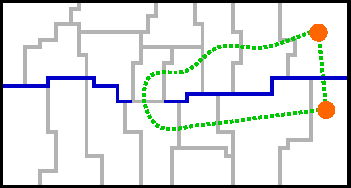
\includegraphics[width=0.4\textwidth]{fig/andres/ineq_0.pdf}
}
\subfloat[Corresponding Graph]{ \label{fig:ineq_1}
    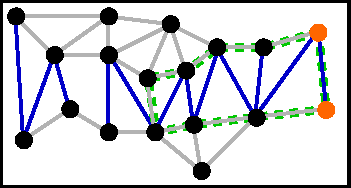
\includegraphics[width=0.4\textwidth]{fig/andres/ineq_1.pdf}
}
\addtocontents{lof}{%
    \vspace{1cm}
    \protect\centerline{%
        \protect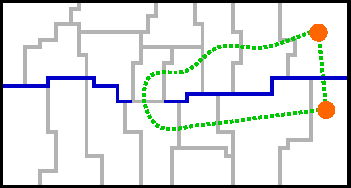
\includegraphics[width=.075\linewidth]{fig/andres/ineq_0.pdf}\hspace{0.2cm}
        \protect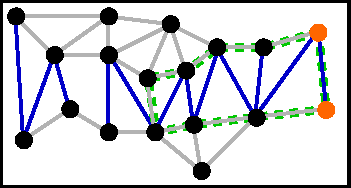
\includegraphics[width=.075\linewidth]{fig/andres/ineq_1.pdf}
    }%
}%
\caption[Violated multicut constraints]{
This figure has been taken from \cite{andres_2011_iccv} .
\Cref{fig:mc_ineq_0} shows the oversegmentation of 
an image .
\Cref{fig:mc_ineq_1} shows the corresponding graph.
} \label{fig:mc_ineq}
\end{figure}

